\documentclass[convert={outfile=\jobname.svg}]{standalone}
\usepackage[dvipsnames]{xcolor}
\usepackage{tikz}
\tikzset{dot/.style={draw,shape=circle,fill=black,scale=0.4}}
\usepackage[outline]{contour}
\contourlength{0.05em}
\newcommand{\outline}[1]{\contour*{white}{#1}}

\begin{document}
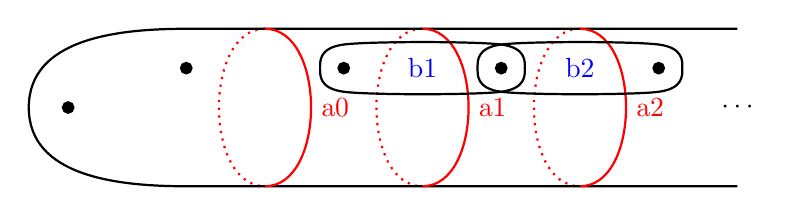
\begin{tikzpicture}[scale=2, thick]
    
    \draw [red, dotted] (1.5, 0.5) to [out=180,in=180] (1.5, -0.5);
    \draw [red, dotted] (2.5, 0.5) to [out=180,in=180] (2.5, -0.5);
    \draw [red, dotted] (3.5, 0.5) to [out=180,in=180] (3.5, -0.5);
    
    \draw (4.5, 0.5) to (1, 0.5) to [out=180,in=90] (0, 0) to [out=270,in=180] (1, -0.5) to (4.5, -0.5);
    \node [dot] at (0.25, 0) {};
    \node [dot] at (1, 0.25) {};
    \node [dot] at (2, 0.25) {};
    \node [dot] at (3, 0.25) {};
    \node [dot] at (4, 0.25) {};
    
    \draw [red] (1.5, 0.5) to [out=0,in=0] node [right] {a0} (1.5, -0.5);
    \draw [red] (2.5, 0.5) to [out=0,in=0] node [right] {a1} (2.5, -0.5);
    \draw [red] (3.5, 0.5) to [out=0,in=0] node [right] {a2} (3.5, -0.5);
    
    \foreach \i in {1, 2} {
        \draw plot [blue, smooth cycle] coordinates {(\i-0.15+1, 0.25) (\i+1, 0.4) (\i+2, 0.4) (\i+2.15, 0.25) (\i+2, 0.1) (\i+1, 0.1)};
        \node [blue] at (\i+1.5, 0.25) {b\i};
    }
    
    \node at (4.5, 0) {$\cdots$};
    
\end{tikzpicture}
\end{document}
